\documentclass[review,3p,times]{elsarticle}
\usepackage[utf8]{inputenc}
\usepackage{amsmath,amssymb}
\usepackage{booktabs}
\usepackage{graphicx}
\usepackage[hidelinks,hypertexnames=false,bookmarks=false]{hyperref}
\graphicspath{{images/}}
\usepackage{array}
\setlength{\emergencystretch}{2em}
\journal{Knowledge-Based Systems}
\hypersetup{pdftitle={Beyond the Random Walk: Horizon-Weighted Temporal Fusion Transformers for Thai Agricultural Commodity Price Forecasting},pdfauthor={Walaiporn Sornkliang, Auyporn Chukeaw, Munlika Rattaphun, Rattayagon Thaiphan, Kritaphat Songsri-in}}
\begin{document}
\begin{frontmatter}
\title{Beyond the Random Walk: Horizon-Weighted Temporal Fusion Transformers for Thai Agricultural Commodity Price Forecasting}
\author[a]{Walaiporn Sornkliang}
\author[a]{Auyporn Chukeaw}
\author[a]{Munlika Rattaphun}
\author[a]{Rattayagon Thaiphan}
\author[a]{Kritaphat Songsri-in\corref{cor1}}
\affiliation[a]{organization={Department of Computer Science, Faculty of Science and Technology, Nakhon Si Thammarat Rajabhat University}, addressline={1 Moo 4, Tha Ngio}, city={Mueang Nakhon Si Thammarat}, postcode={80280}, state={Nakhon Si Thammarat}, country={Thailand}}
\cortext[cor1]{Corresponding author. E-mail: kritaphat\_son@nstru.ac.th}
\begin{abstract}
Forecasting agricultural commodity prices is difficult because non-stationarity and low signal-to-noise ratios often cause high-capacity models to lose to persistence. We evaluate one global Temporal Fusion Transformer (TFT) across 404 Thai crop products at four horizons ($t+20$, $t+60$, $t+120$, and $t+250$ business days). Motivated by the mismatch between uniform decoder-step weighting and horizon-dependent forecast difficulty, we introduce a \textbf{Horizon-Weighted Quantile Loss}, $w(h)=1/h^\gamma$. A sweep of seventeen decay exponents ($\gamma \in [0,8]$) reveals a broad low-error region, and a single $\gamma=4.5$ model is selected using the held-out 2023 validation year. On matched 2024--2025 test windows, the selected model improves every aggregate metric over Lag-1 persistence: MAE \textbf{39.76 versus 45.21 THB (12.0\% lower)}, SMAPE \textbf{0.7\% lower}, and RMSE \textbf{15.1\% lower}. The gain is concentrated at one year (\textbf{36.8\% lower MAE}), whereas the model underperforms at $t+20$ (26.51 versus 15.11 THB). Product-clustered tests identify both differences as significant after Holm correction ($p<0.01$), and the per-crop win rate is \textbf{57.7\%}. Results hold against seasonal-naive, drift, and zero-shot foundation-model baselines and across three training seeds. Validation-fitted conformal-style scaling gives 78--90\% empirical coverage for nominal 80\% intervals. A persistence-anchored ensemble variant reaches \textbf{36.04 THB} overall without underperforming persistence at any reported horizon on this test set.

\end{abstract}
\begin{keyword}
Multi-horizon time series forecasting \sep Temporal Fusion Transformer \sep Agricultural commodity prices \sep Horizon-weighted loss \sep Quantile regression \sep Prediction interval calibration
\end{keyword}
\end{frontmatter}

\section{Introduction}

Agricultural commodity markets in developing nations, particularly Thailand, are characterized by high price volatility. As a leading exporter of rice, cassava, and other crops, Thailand's economic stability is tied to agricultural pricing. However, these prices are subject to complex domestic supply shocks, international trade policies, and market inefficiencies. Reliable price forecasting over multiple horizons is essential for risk mitigation, farm-level decision-making, and policy formulation.

Under the efficient market hypothesis, agricultural asset prices are theorized to follow random walks, rendering historical price-only structures uninformative for future horizons. Empirically, this is reflected in the difficulty that high-capacity models encounter when trying to outperform naive local baselines out-of-sample. This phenomenon, which we term 'architectural saturation,' arises because complex neural architectures (e.g., standard sequence-to-sequence Transformers, deep MLPs, and recurrent networks) possess high parameter density and capacity, allowing them to fit arbitrary functions. However, agricultural price series are characterized by low signal-to-noise ratios, non-stationarity, and frequent structural breaks. When trained on such series, high-capacity models tend to memorize transient noise and spurious historical correlations within the training sample rather than extracting persistent, structural patterns. Consequently, when evaluated on out-of-sample hold-out periods (such as 2024--2025), these over-parameterized models suffer from generalization collapse, performing significantly worse than a simple Lag-1 persistence model, which remains robust due to its zero-parameter simplicity.

To overcome the limitations of localized statistical modeling and mitigate the risk of architectural saturation, we employ cross-product representation learning using a global Temporal Fusion Transformer (TFT) architecture. Traditional local models are trained independently on each of the 404 crops, meaning they cannot share statistical strength and are highly vulnerable to localized data scarcity or reporting anomalies. In contrast, our global modeling framework pools the price histories of all 404 crops into one training dataset and fits a single set of shared model parameters. To prevent the model from conflating different crop dynamics, we supply static variables (product, category, and group identifiers) to a static covariate encoder, mapping them to low-dimensional embedding spaces. This representation learning paradigm allows the TFT to capture shared functional structure while conditioning forecasts on entity-specific embeddings. The pooling claim does not rest on correlated prices: supplementary diagnostics show weak average co-movement across the 404 crops (0.18 in levels and 0.012 in daily returns).

Importantly, the scope of our claim is bounded. Under a martingale model persistence is mean-squared-error optimal, and under symmetric increments it is also optimal for absolute error; our experiments likewise show that no pooled neural configuration approaches it at $t+20$. The proposed model, a single horizon-weighted TFT, therefore concedes the near-term regime to persistence and overtakes it from six months onward, where random-walk forecast variance accumulates and slower structure can become useful. We also document a persistence-anchored ensemble variant that avoids horizon-level degradation on this test set, while not claiming that validation-fitted weights guarantee future performance.

The primary contributions of this paper are:
\begin{enumerate}
\item We establish a multi-scale forecasting evaluation targeting four distinct future horizons: $t+20$ (one business month), $t+60$ (three business months), $t+120$ (six business months), and $t+250$ (one business year), with model and baseline forecasts compared on identical test windows.
\item We formulate horizon allocation in joint sequence prediction explicitly and introduce a Horizon-Weighted Quantile Loss parameterized by the power-law family $w(h) = 1/h^\gamma$. A controlled seventeen-point sweep maps the full empirical trade-off over $\gamma \in [0, 8]$: near-term error falls by nearly two-thirds within a broad low-error region, while one-year accuracy and raw interval quality deteriorate when far-horizon supervision becomes negligible.
\item We select the operating point ($\gamma = 4.5$) by error on a held-out validation year rather than on the test set, and report the resulting single model together with an explicit accounting of where and how much it improves on the naive baseline.
\item We show that the selected model reduces matched out-of-sample error against the Lag-1 baseline on every aggregate metric (MAE -12.0\%, SMAPE -0.7\%, RMSE -15.1\%, and by 36.8\% MAE at one year), report validation-fitted interval scaling (78--90\% empirical coverage), and document ensembling and persistence-anchored variants that trade simplicity for improved horizon-level robustness.
\item We test the horizon-level differences with product-level one-sample t-tests and Wilcoxon signed-rank tests, control the four horizon-wise comparisons with Holm's procedure, repeat the selected exponent under three seeds, and compare against seasonal-naive, drift, and zero-shot foundation-model baselines.

\end{enumerate}
The remainder of this paper is structured as follows. Section 2 reviews related work. Section 3 details the dataset and exploratory data analysis. Section 4 describes the methodology, including the evaluation protocol, the TFT architecture, the horizon-weighted loss, and the model-selection procedure. Section 5 presents the quantitative results. Section 6 discusses model interpretability. Section 7 evaluates probabilistic calibration, and Section 8 concludes.

\section{Related Work}

Historically, agricultural price forecasting has been dominated by localized, parametric statistical models. The Autoregressive Integrated Moving Average (ARIMA) framework, popularized by Box and Jenkins [1], serves as a classical benchmark. These local models are fitted independently to each individual commodity series under the assumption of linear, stationary data-generating processes. While ARIMA and its seasonal variants (SARIMA) provide robust predictions in stable economic regimes, they fail to capture the high-frequency non-linear dynamics, volatility clustering, and sudden structural breaks characteristic of developing agricultural markets [2]. Furthermore, because these statistical methods are localized, they cannot share parameters across different commodities. This severely limits their predictive capacity when individual series are short, incomplete, or characterized by low signal-to-noise ratios.

To capture non-linear relationships, researchers transitioned to machine learning (ML) paradigms, such as Support Vector Regression (SVR), Random Forests, and Gradient Boosting Decision Trees (GBDT), including XGBoost and LightGBM. GBDTs have shown strong empirical performance on tabular forecasting tasks [3] due to their ability to construct non-linear decision boundaries. Tree ensembles have also been applied to this particular market. A random forest fitted to monthly vegetable prices in Nakhon Si Thammarat Province forecast individual crops with low percentage error [4], though one crop at a time on monthly aggregates, without the pooled cross-product structure, the daily sampling, or the multi-horizon evaluation protocol studied here. However, standard ML models treat sequence prediction as a static regression problem, requiring extensive manual feature engineering of rolling windows and historical lags. In a global setting, where a single model is trained across a diverse cross-section of products, traditional GBDTs struggle to scale efficiently. They often experience severe overfitting to localized noise rather than learning generalizable sequential relationships, a precursor to architectural saturation out-of-sample.

The advent of deep learning (DL) provided a framework for end-to-end representation learning. Recurrent Neural Networks (RNNs), particularly Long Short-Term Memory (LSTM) networks [5] and Gated Recurrent Units (GRUs), introduced gated cell states to capture sequential dependencies. While RNNs address sequence learning, they suffer from vanishing gradients over long lookback windows and process inputs sequentially, which limits parallelization during training. The self-attention mechanism of the Transformer [6] resolved these bottlenecks, enabling the modeling of long-range interactions. Nevertheless, standard Transformers are highly over-parameterized and lack specialized mechanisms to handle the distinct properties of time-series data, such as static metadata and time-varying covariates, often resulting in architectural saturation where the model overfits to historical noise and fails to generalize out-of-sample.

To bridge this gap, the Temporal Fusion Transformer (TFT) was developed [7]. The TFT combines self-attention with Gated Residual Networks (GRN) and Variable Selection Networks (VSN). The VSN acts as an active information filter, selecting relevant features at each step, while the GRN provides adaptive model capacity by bypassing unnecessary layers. This architectural flexibility is critical for agricultural price forecasting, where the signal-to-noise ratio is low and overfitting is common. Furthermore, the TFT introduces interpretable self-attention, allowing researchers to inspect the exact historical steps the model prioritized when generating forecasts. Similar architectures, such as PatchTST [8] and iTransformer [9], have focused on channel-independence or patching to capture local sequences. However, they lack the native integration of static metadata (e.g., crop class, market category) and dynamic covariates in a unified framework, which is crucial for transfer learning across heterogeneous agricultural markets. Similarly, large pre-trained foundation models like Chronos [10] perform zero-shot forecasting, but they can produce spurious long-horizon trajectories when decoupled from localized, entity-specific economic context.

Finally, our system design draws on two classical strands of the forecasting literature. Forecast combination, averaging or convexly weighting heterogeneous forecasters, has been shown to improve accuracy and robustness since Bates and Granger [11], and combination strategies have dominated recent large-scale forecasting competitions such as M4 and M5 [12]. Deep ensembles [13] similarly average independently trained networks to reduce the variance intrinsic to stochastic gradient training. Our persistence-anchored ensemble applies both ideas jointly: an ensemble across loss-weighting configurations to suppress training variance, and a convex combination with the naive persistence forecast to reduce exposure to the near-term random-walk regime.

For probabilistic forecasts, conformalized quantile regression combines learned quantile intervals with held-out nonconformity scores and can provide finite-sample marginal coverage under exchangeability and a calibration split independent of model fitting [14]. Agricultural price windows violate the simplest version of those conditions because adjacent origins overlap and the 2023 validation labels also guide early stopping and model selection. We therefore use the same score construction only as a \emph{conformal-style, validation-fitted interval rescaling} and evaluate its realized test coverage; we do not claim a distribution-free conformal guarantee.

\section{Data and Exploratory Analysis}

Our dataset comprises daily minimum and maximum price recordings for \textbf{729 agricultural products} in Thai markets, obtained from the Ministry of Commerce (Thailand), Department of Internal Trade, via its public Open Data portal [15], spanning January 2018 through December 2025 on a Monday--Friday business calendar (2,086 business days). Each product carries a product identifier, a retail/wholesale category, and a commodity group. All summaries were regenerated by \texttt{run\_eda.py}, and the per-product profile is released as \texttt{eda\_product\_summary.csv}.

Zero and anomalous reports are treated as missing, rolling-IQR outliers are removed, gaps are forward-filled after alignment to a business-day calendar, and products without sufficient price variation are excluded. Of 729 raw products, 635 contain active observations and 404 satisfy the modeling filter. The retained series are highly persistent in levels, heterogeneous in long-run trends, and weakly correlated in daily returns (mean pairwise return correlation 0.012). Full group counts, stationarity tests, ACF/PACF summaries, trend plots, and co-movement diagnostics are reported in the Supplementary Material so the main paper can focus on the forecasting experiment.

\setcounter{table}{2}

\section{Methodology}

\subsection{Forecasting Horizons and Evaluation Metrics}
We establish a multi-scale forecasting horizon aligned with agricultural decision cycles. Given the input sequence, models forecast at specific future steps:
\begin{itemize}
\item $t+20$: One business month / 20 business days.
\item $t+60$: Three business months / 60 business days.
\item $t+120$: Six business months / 120 business days.
\item $t+250$: One business year / 250 business days.

\end{itemize}
Performance is measured using Mean Absolute Error (MAE), Root Mean Squared Error (RMSE), and Symmetric Mean Absolute Percentage Error (SMAPE), calculated as:

\[\text{MAE} = \frac{1}{N} \sum_{i=1}^{N} |y_i - \hat{y}_i|\]

\[\text{RMSE} = \sqrt{\frac{1}{N} \sum_{i=1}^{N} (y_i - \hat{y}_i)^2}\]

\[\text{SMAPE} = \frac{100\%}{N} \sum_{i=1}^{N} \frac{|y_i - \hat{y}_i|}{(|y_i| + |\hat{y}_i|)/2}\]

where $y_i$ represents the actual price and $\hat{y}_i$ represents the predicted price. For every quantile-regression TFT in this study (Section 4.4, item 5), $\hat{y}_i$ is the network's median (0.5 quantile) output, $\hat{y}^{med}_i$ in the notation of Section 4.7; the 0.1 and 0.9 quantile heads contribute only to the prediction intervals of Section 7 and never to the point-forecast metrics reported in Tables 5 through 8. For the non-quantile reference models of Section 4.3, $\hat{y}_i$ is each model's single point output.

\subsection{Evaluation Protocol and Matched-Sample Comparison}

All results follow a strict out-of-time protocol, summarized in Table 3. Model parameters are learned on labels through the end of 2022 over the pooled 404-crop dataset; the 2023 calendar year serves as the validation period for early stopping and for fitting all post-hoc calibration parameters; the 2024--2025 period is reserved exclusively for final evaluation. For every forecast origin in the test period, the model and the Lag-1 persistence baseline are evaluated on the \emph{identical} window, with the persistence forecast defined as the final observed value of that window's encoder segment. This matched-sample design eliminates a subtle but serious failure mode in which model and baseline metrics are computed over different origin distributions and become incomparable. Each of the four reporting horizons is evaluated over 110,292 test windows (273 origins for each of the 404 crops); because every crop contributes an identical number of windows, the pooled average coincides exactly with the per-product macro-average. Validation-side fitting of calibration (and blend-variant) parameters uses, per horizon, every window whose label at that horizon falls within 2023 (12,120 windows at $t+20$ growing to 105,040 at $t+250$), so that even the longest horizon is fitted on a full year of labels rather than a small number of early-year origins.

\begin{table}[htbp]\centering
\caption{Chronological Data Partition and Its Role in the Protocol. Validation labels serve early stopping, decay-exponent selection, interval calibration, and blend-weight fitting; no test-period information enters any fitted quantity}
\small
\begin{tabular}{llll}
\toprule
Partition & Period & Labels used for & Windows per horizon \\
\midrule
Training & 2018--2022 & Parameter estimation (404 crops, pooled) & n/a \\
Validation & 2023 & Early stopping; selection; calibration & 12,120--105,040 \\
Test & 2024--2025 & Final evaluation only & 110,292 \\
\bottomrule
\end{tabular}
\end{table}

\subsection{Baseline and Reference Models}

We compare the proposed model against a suite of localized statistical benchmarks and global machine learning and deep learning references. The suite is constructed so that the comparisons of Section 5 isolate four distinct questions: whether any classical local rule, naive or fitted, is hard to beat (persistence, seasonal-naive, drift, and ARIMA), whether pooled learning over engineered features adds value without any sequence modeling (LightGBM), whether increasing architectural capacity adds value under identical inputs (MLP, gated recurrent networks, and a standard Transformer), and whether large-scale pretraining on heterogeneous time series substitutes for in-domain training (a zero-shot foundation model). All learned references share the conditions described below, so that differences in Table 5 are attributable to model class rather than to data, features, or evaluation.

Every in-domain learned reference uses the same leakage-safe price-lag, return, rolling-statistic, repricing, calendar, and entity features and is fitted through 2023 before evaluation on the identical 2024--2025 windows. LightGBM uses direct horizon-specific regression; the MLP, LSTM, and Transformer use joint multi-output regression; ARIMA is fitted per product; and Chronos-Bolt-Base is evaluated zero-shot from up to 512 prior observations. Detailed equations, configurations, and a ten-candidate validation search for each learned reference are provided in the Supplementary Material. Table 5 retains the original configurations, while the supplement shows that no validation-selected alternative beats persistence overall or approaches the selected TFT.

For the primary selected-TFT comparison, overlapping daily origins preclude treating window errors as independent. We therefore average the absolute-error differential within each product and apply a two-sided one-sample t-test and Wilcoxon signed-rank test to the 404 product means. Holm's procedure controls the four horizon-wise tests separately for each test family; the pre-specified overall contrast is reported separately. Mean cross-product return correlation is low, but residual dependence among near-duplicate products remains a limitation.


\subsection{Temporal Fusion Transformer Architecture}

The Temporal Fusion Transformer (TFT) architecture integrates static metadata and multi-scale sequential covariates using specialized neural blocks. The network is optimized end-to-end to generate multi-horizon probabilistic forecasts. All inputs to the TFT in our experiments are strictly price-derived (the historical target series) plus deterministic calendar covariates and categorical metadata (product, category, and market group IDs).

Information flows through the network as follows. Static metadata is mapped to entity embeddings and then to context vectors that condition downstream blocks. At each time step, a variable selection network weighs the available inputs; the selected representation passes through an LSTM encoder over the 30-day lookback window and an LSTM decoder over the 250-step forecast window, both initialized from static context. Gated skip connections and interpretable multi-head self-attention enrich the decoder states, and linear quantile heads emit the 10th, 50th, and 90th percentile forecasts at every decoder step under the horizon-weighted loss of Section 4.5. Table 4 consolidates the configuration.

The Supplementary Material gives the GRN, VSN, LSTM, shared-value attention, and pinball-loss equations. In the interpretable attention block, query and key projections are head-specific, the value projection is shared, and head attention matrices are averaged [7].


\subsubsection{Training Configuration and Hyperparameters}
Table 4 consolidates the complete configuration, which is identical for every TFT in this study; the decay exponent $\gamma$ of the loss function (Section 4.6) is the only quantity varied across experiments, so that any performance difference in Section 5.2 is attributable to the loss geometry alone. All experiments are conducted globally over the pooled crop dataset with a fixed random initialization per run and are accelerated with PyTorch and CUDA on dedicated GPU hardware (NVIDIA RTX series). The full training and evaluation pipeline, including per-run artifacts (metrics, per-sample predictions, and model checkpoints), is reproducible from the accompanying code.

\begin{table}[htbp]\centering
\caption{Temporal Fusion Transformer Configuration (identical across all experiments)}
\small
\begin{tabular}{ll}
\toprule
Component & Setting \\
\midrule
Encoder (lookback) length & 30 business days \\
Decoder (forecast) length & 250 business days; reporting horizons $t+20$, $t+60$, $t+120$, $t+250$ \\
Hidden state size & 64 \\
Attention heads & 4 \\
Continuous-variable encoding size & 8 \\
Dropout & 0.1 \\
Output quantiles & $\{0.1, 0.5, 0.9\}$ \\
Target normalization & Per-product group normalizer, softplus transformation \\
Loss function & Horizon-Weighted Quantile Loss, $w(h) = 1/h^\gamma$ (Section 4.6) \\
Optimizer & Adam, learning rate 0.01, reduce-on-plateau schedule (patience 4) \\
Batch size & 64 (training), 128 (inference) \\
Gradient clipping & 0.1 \\
Epoch budget & 5, with early stopping on validation loss (patience 5, min. delta $10^{-4}$) \\
\bottomrule
\end{tabular}
\end{table}

\setcounter{subsection}{5}

\subsection{Horizon Allocation and the Horizon-Weighted Quantile Loss}

A standard joint decoder objective averages losses uniformly over all 250 forecast steps. Uniform per-step weighting is not neutral when the application values a small set of decision horizons: 230 of the 250 terms lie beyond the first business month, and expected forecast loss generally grows with horizon. The resulting objective therefore allocates most of its total loss mass to a long block of distant steps, even though early and distant steps can favor different parameter updates.

This statement concerns \emph{loss allocation}, not a directly measured increase in per-residual gradient magnitude. For pinball loss $\rho_q(u)=u(q-\mathbb{1}\{u<0\})$, the subgradient with respect to the prediction is bounded:
$$\frac{\partial \rho\_q(y-\hat y)}{\partial \hat y} =
\begin{cases}
-q, \& y>\hat y,\\
1-q, \& y<\hat y.
\end{cases}$$
Its magnitude does not grow with the absolute residual. We therefore do not infer gradient dominance merely from larger far-horizon errors, nor do we measure gradient-vector conflict directly. Instead, we test the narrower empirical hypothesis that explicitly reallocating the joint objective across decoder steps changes the multi-horizon accuracy trade-off.

We apply a step-dependent weight $w(h)$ to the quantile loss at every decoder step:
\[\mathcal{L}_{HW\text{-}Quantile} = \sum_{h=1}^{H} w(h) \cdot \mathcal{L}_{Quantile}(y_{pred, t+h}, y_{true, t+h})\]

We parameterize the loss decay weighting function using a 1-parameter power-law family:
\[w(h) = \frac{1}{h^\gamma}\]
where $\gamma \ge 0$ controls how rapidly loss contributions from later decoder steps are discounted.

We adopt a power-law family for three reasons. First, a single-exponent power law is scale-free: rescaling the horizon by a constant rescales all weights by a common factor, whereas an exponential schedule introduces an additional characteristic decay horizon. Second, it provides a one-parameter path from the unweighted objective ($\gamma=0$) to increasingly early-focused training. This fixed modulation is analogous in spirit to focal reweighting [18] and is simpler to audit than adaptive multi-task schemes such as GradNorm [19]. Third, under a zero-drift random walk, persistence error has variance $\text{Var}(y_{t+h}-y_t)=h\sigma^2$ [1], so expected absolute error and expected pinball-loss scale grow as $\mathcal{O}(\sqrt{h})$ under symmetric innovations. Thus $\gamma=0.5$ approximately normalizes the \emph{expected loss scale} across horizons in that stylized case; it does not normalize the bounded pinball subgradient itself.

Under this formulation, we systematically evaluate seventeen decay exponents spanning $\gamma \in \{0.0, 0.5, \dots, 8.0\}$ in half-unit steps, ranging from the standard unweighted objective ($\gamma = 0$, $w(h) = 1$) through square-root, linear, and inverse-square decays to extreme early-step prioritization (at $\gamma = 8$ the weight on the 250th step is of order $10^{-20}$). Representative weight curves are shown in the Supplementary Material.


\subsection{Model Selection, Seed Sensitivity, and Interval Calibration}

\textbf{1. Model selection on validation.} The seventeen-point sweep uses seed 42 for every candidate. We select the decay exponent with the lowest mean MAE across the four reporting horizons on the 2023 validation year; $\gamma = 4.5$ is the minimum. Test metrics do not enter this formal selection rule. After fixing the exponent, we retrain it under seeds 43 and 44 as a sensitivity analysis rather than averaging seeds into the selection criterion. Across the three runs, overall test MAE ranges from 39.76 to 43.70 THB versus 45.21 THB for persistence; all three runs retain the $t+120$ and $t+250$ advantage. The selected seed-42 artifact supplies the primary tables, while the full multi-seed results are reported in the Supplementary Material.

\textbf{2. Validation-fitted conformal-style interval scaling.} Raw quantile intervals from pooled TFTs are systematically too narrow on this data, increasingly so at steep decay exponents whose vanishing far-future loss weights leave dispersion weakly supervised. Inspired by locally adaptive conformalized quantile regression [14], we rescale the 80\% interval around the median by a per-horizon factor $s_h$, chosen as the empirical 80th percentile of the validation nonconformity scores
\[r_i = \max\!\left(\frac{\hat{y}^{med}_i - y_i}{\hat{y}^{med}_i - \hat{y}^{lo}_i}, \; \frac{y_i - \hat{y}^{med}_i}{\hat{y}^{hi}_i - \hat{y}^{med}_i}\right)\]
so that the scaled interval $[\hat{y}^{med} - s_h(\hat{y}^{med} - \hat{y}^{lo}), \; \hat{y}^{med} + s_h(\hat{y}^{hi} - \hat{y}^{med})]$ attains approximately nominal empirical coverage on validation. Scales are fitted per horizon on all windows whose horizon-$h$ label falls in 2023; no test-period information enters the scale. This is not a formal split-conformal construction: the same validation year also informs early-stopping monitoring and exponent selection, adjacent windows overlap, and temporal exchangeability is implausible. Accordingly, Section 7 reports empirical test coverage without a finite-sample guarantee.

\textbf{3. System variants for comparison.} Because forecast combination is the classical remedy for both training variance and near-term weakness [11,13], we also evaluate two variants: (i) a \emph{gamma-ensemble} that averages the median forecasts of the moderate-decay members, $\hat{y}^{ens}_{t+h} = \frac{1}{|\Gamma|}\sum_{\gamma \in \Gamma} \hat{y}^{(\gamma)}_{t+h}$ with $\Gamma = \{0.0, 0.5, \dots, 3.0\}$ selected on validation; and (ii) a \emph{persistence-anchored} blend $\hat{y}^{sys}_{t+h} = \alpha_h \hat{y}^{ens}_{t+h} + (1-\alpha_h) y_t$ with per-horizon convex weights fitted on 2023 validation MAE. Since $\alpha_h = 0$ recovers the baseline exactly, the anchored variant is never worse than persistence by construction on validation; its test behavior is reported in Section 5.3.

\subsection{Target-Normalizer Staleness Diagnostic}

The per-product \texttt{GroupNormalizer} is fitted on 2018--2022 and not refreshed. As an exploratory diagnostic, a raw-price proxy for the level shift from the training-period mean to the final 2023 observation exceeds 10\% for 70.6\% of products and correlates with relative $t+20$ error (Spearman $r=0.146$, unadjusted $p=0.007$). Because the proxy is not the transformed internal normalizer center and the association is not causal, full definitions, quartile results, and long-horizon correlations are placed in the Supplementary Material.



\section{Quantitative Results}

This section reports results in the order of the questions posed in Section 4.3. Section 5.1 establishes the reference comparison across model classes; Section 5.2 maps the effect of the decay exponent on accuracy and interval quality; Section 5.3 evaluates the validation-selected model against the matched baseline, including its temporal stability and the system variants; and Section 5.4 examines individual forecast trajectories qualitatively. All numbers follow the matched-window protocol of Section 4.2, and, unless stated otherwise, aggregate figures average the four reporting horizons over the full 2024--2025 test period.

\subsection{Reference Benchmark Suite}

Table 5 reports a broad model comparison across local statistical benchmarks, pooled global learners, and a zero-shot foundation model, all evaluated under the matched-window protocol of Section 4.2: the same 404 crops, the same 110,292 test windows per horizon, and the same baseline as every other table in this paper. The last two rows report a standard unweighted TFT control and the selected horizon-weighted model defined in Section 4.7.

Four patterns emerge. First, no classical local rule improves on persistence overall. ARIMA is numerically indistinguishable from it; seasonal-naive is substantially worse (70.19 THB overall); and drift is worse at every horizon beyond $t+20$ (49.90 THB overall). Second, the global MLP, LSTM, Transformer, and unweighted TFT are worse than persistence overall, whereas LightGBM is competitive (44.83 THB). Third, zero-shot Chronos-Bolt reaches 47.01 THB, competitive with but not better than persistence on this dataset. This is a result for one foundation-model checkpoint and zero-shot protocol, not a general claim about pretrained forecasters. Fourth, holding the TFT architecture, data, seed, and training budget fixed, horizon weighting changes its overall MAE from 72.85 to 39.76 THB and yields the best $t+120$ and $t+250$ values in Table 5. This controlled contrast is consistent with loss allocation being a key constraint in the unweighted TFT; it does not isolate every possible architecture or optimization explanation.

\begin{table}[htbp]\centering
\caption{Reference Suite Mean Absolute Error by Horizon (THB; matched-window protocol, 404 crops)}
\small
\begin{tabular}{lccccc}
\toprule
Model & $t+20$ & $t+60$ & $t+120$ & $t+250$ & Overall \\
\midrule
Lag-1 Persistence & \textbf{15.11} & \textbf{30.86} & 51.03 & 83.84 & 45.21 \\
Seasonal-Naive & 62.18 & 63.76 & 71.00 & 83.84 & 70.19 \\
Drift & 15.69 & 32.70 & 55.76 & 95.47 & 49.90 \\
ARIMA & 15.11 & 30.87 & 51.02 & 83.83 & 45.21 \\
Global LightGBM & 29.37 & 43.37 & 49.69 & 56.88 & 44.83 \\
Global MLP & 46.34 & 48.22 & 53.34 & 79.60 & 56.88 \\
Global LSTM & 50.68 & 51.43 & 56.65 & 79.60 & 59.59 \\
Global Transformer & 46.71 & 57.22 & 74.80 & 104.55 & 70.82 \\
Chronos-Bolt (zero-shot) & 16.85 & 33.85 & 53.37 & 83.98 & 47.01 \\
TFT & 69.74 & 76.37 & 73.94 & 71.37 & 72.85 \\
\textbf{Horizon-Weighted Quantile TFT (ours)} & 26.51 & 33.81 & \textbf{45.75} & \textbf{52.97} & \textbf{39.76} \\
\bottomrule
\end{tabular}
\end{table}

\subsection{Loss Decay Exponent ($\gamma$) Sweep}

Figure 6 plots horizon-specific and overall test MAE for one matched seed-42 run per exponent; the full numeric grid is in the Supplementary Material. High decay generally improves near-term accuracy relative to the unweighted objective, but the path is not monotone. Raw $t+20$ MAE falls from 69.74 THB at $\gamma=0$ to 23--30 THB for most $\gamma \ge 4$ (minimum 22.80 at $\gamma=6.5$), a reduction of up to \textbf{67\%} under otherwise identical architecture, data, seed, and training budget. Overall test MAE occupies a broad but noisy low-error region of 39.76--48.63 THB for $\gamma \in [3,6]$; validation MAE selects $\gamma=4.5$. For $\gamma \in [6.5,8]$, one-year MAE is 67--71 THB, consistent with excessively weak far-horizon supervision. Because each grid point is a single run, fine-grained non-monotonic differences should not be read as a smooth dose-response curve.

\setcounter{table}{6}
\setcounter{figure}{5}

\begin{figure}[htbp]\centering
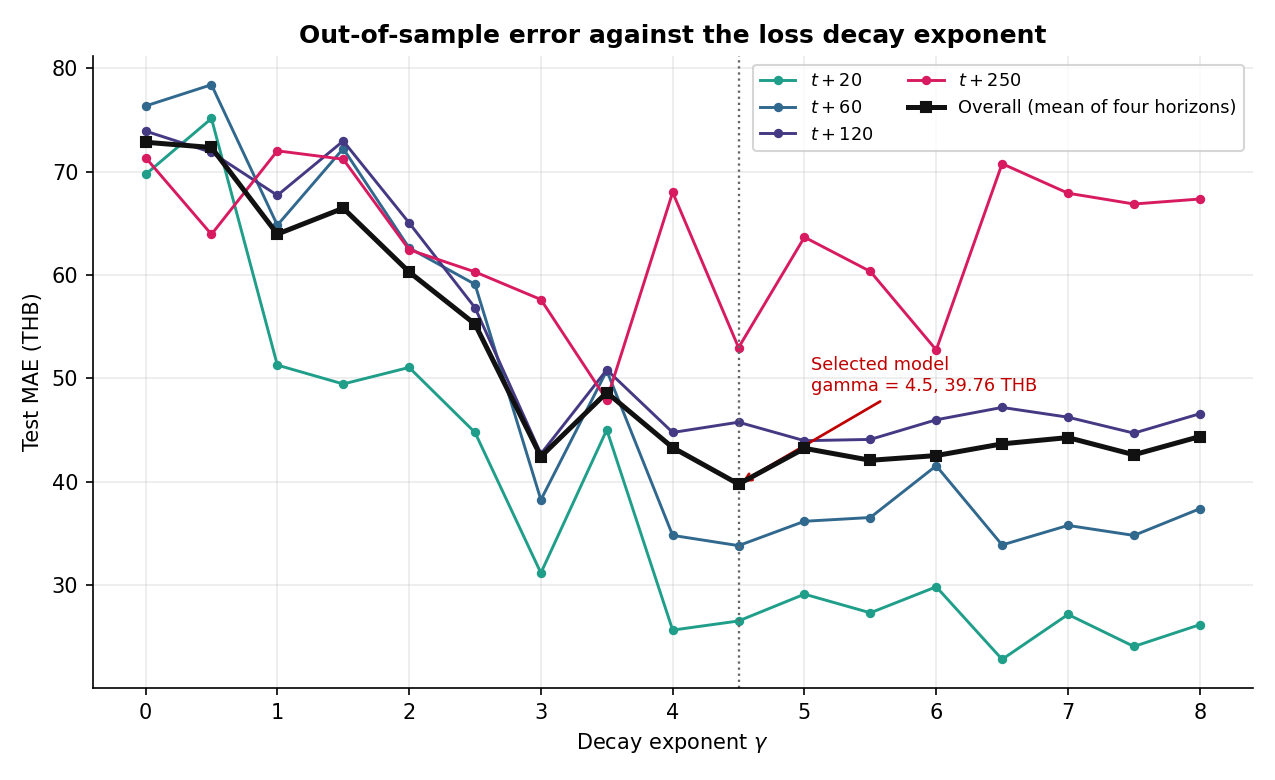
\includegraphics[width=\linewidth]{mae_vs_gamma.png}
\caption{Horizon-specific and overall test MAE across the power-law decay exponent grid, one seed-42 run per point. Per-column minima in Table 6 are bolded.}
\end{figure}

Two properties of this region govern the choice of operating point. First, $\gamma = 4.5$ attains the lowest validation MAE of any swept exponent and is therefore selected (Section 4.7); its test performance is reported in Section 5.3. The three-seed sensitivity analysis gives overall MAE of 39.76, 42.22, and 43.70 THB, so the exact figure is initialization-dependent even though the aggregate and long-horizon ranking against persistence is stable across those runs.

Second, raw probabilistic quality generally deteriorates as decay becomes steep. Across horizons, raw 80\% interval coverage ranges from 38--65\% for the shallower members ($\gamma \le 3$) and reaches values as low as 6.3\% for $\gamma \ge 6$. The association is not strictly monotone at every grid point, but it is consistent with weakly weighted outer quantile heads learning inadequate far-horizon spread. Operational use of the selected model therefore requires separately validated interval scaling; point accuracy alone does not justify its raw intervals.

\subsection{Selected Model Performance}

Table 7 reports the selected horizon-weighted TFT ($\gamma = 4.5$) against the matched Lag-1 baseline. It improves every aggregate metric: MAE by 12.0\%, SMAPE by 0.7\%, and RMSE by 15.1\%. The gains are concentrated precisely where theory predicts: -10.3\% MAE at six months and -36.8\% at one year, as accumulated drift variance degrades the random-walk forecast. The trade-off is reported explicitly rather than obscured by the aggregates. The selected model remains behind the baseline at $t+20$ (26.51 vs 15.11 THB) and $t+60$ (33.81 vs 30.86 THB), where daily price changes are near-unpredictable and the persistence rule is close to optimal.

Every horizon-level difference in Table 7 is tested on the 404 product-level mean differentials using a one-sample t-test and Wilcoxon signed-rank test. Raw values are shown in the table. After Holm correction across the four horizons, the $t+20$ deficit, $t+120$ gain, and $t+250$ gain remain significant on both tests (adjusted t-test $p=0.0028$, $0.0019$, and $0.0009$, respectively; adjusted Wilcoxon $p<10^{-9}$ in each case). The $t+60$ difference remains non-significant (adjusted $p=0.091$ and $0.184$). The separately specified overall contrast is also significant on both unadjusted tests ($p=0.0001$ and $p<0.0001$). These results are conditional on treating products as analysis units; residual dependence among near-duplicate series is addressed in the limitations.

\begin{table}[htbp]\centering
\caption{Selected TFT ($\gamma = 4.5$) vs. Matched Lag-1 Baseline. Each cell reports MAE (THB) / SMAPE / RMSE (THB); bold marks the better model per row, negative $\Delta$ favors the selected model, and $p$ is the raw product-level t-test / Wilcoxon significance of the MAE difference (Section 4.3)}
\small
\begin{tabular}{lcccc}
\toprule
Horizon & Baseline & Selected TFT & $\Delta$ (MAE / SMAPE / RMSE) & $p$ (t / Wilcoxon) \\
\midrule
$t+20$ & \textbf{15.11 / 7.59\% / 61.84} & 26.51 / 8.79\% / 116.59 & +75.5\% / +15.8\% / +88.5\% & 0.0014 / $<$0.0001 \\
$t+60$ & \textbf{30.86 / 14.32\% / 118.13} & 33.81 / 14.64\% / 124.44 & +9.5\% / +2.2\% / +5.3\% & 0.091 / 0.184 \\
$t+120$ & 51.03 / 18.23\% / 194.65 & \textbf{45.75 / 17.98\% / 165.49} & \textbf{-10.3\% / -1.4\% / -15.0\%} & 0.0006 / $<$0.0001 \\
$t+250$ & 83.84 / 19.98\% / 330.39 & \textbf{52.97 / 18.29\% / 191.90} & \textbf{-36.8\% / -8.4\% / -41.9\%} & 0.0002 / $<$0.0001 \\
\textbf{Overall} & 45.21 / 15.03\% / 176.25 & \textbf{39.76 / 14.93\% / 149.61} & \textbf{-12.0\% / -0.7\% / -15.1\%} & 0.0001 / $<$0.0001 \\
\bottomrule
\end{tabular}
\end{table}

The RMSE columns extend the comparison to the tail-sensitive metric and sharpen both sides of the trade-off. The selected model's near-term deficit is larger on RMSE than on MAE (+88.5\% against +75.5\% at $t+20$), indicating that its short-horizon errors include occasional large misses, while its long-horizon advantage is correspondingly larger (-41.9\% at one year). Two qualifications place this result in context. First, the aggregate margin on the scale-free metric is thin (SMAPE improves by only 0.7\% overall) and rests entirely on the long horizons. At $t+20$ the selected model is 75.5\% worse on MAE than repeating the most recent observed price. Second, the improvement is not uniform across the cross-section. The selected model outperforms persistence on \textbf{57.7\%} of the 404 individual crops overall (hereafter the per-crop win rate), rising from 24.5\% at $t+20$ to 62.4\% at $t+120$ and 70.3\% at $t+250$. Its aggregate advantage comes from large gains on a subset of series rather than from improving every crop, and approximately two of every five crops are forecast more accurately by the naive rule. The claim advanced in this paper is therefore specific. A single pooled, horizon-weighted TFT decisively outperforms the random walk in aggregate and at extended horizons, while conceding both the near-term regime and a substantial minority of individual series.

Under the stylized zero-drift random walk $y_t=y_{t-1}+\epsilon_t$, $\epsilon_t\sim\mathcal{N}(0,\sigma^2)$, persistence error variance grows as $\text{Var}(y_{t+h}-y_t)=h\sigma^2$ and expected absolute error as $\mathcal{O}(\sqrt{h})$. The empirical baseline MAE likewise rises from 15.11 THB at $t+20$ to 83.84 THB at $t+250$, while the selected model rises from 26.51 to 52.97 THB. This flatter observed curve is consistent with the pooled model exploiting slower shared structure, but the experiment does not identify a unique economic mechanism or prove that its error remains bounded outside the test period.

To verify that the improvement is not an artifact of a particular evaluation period, Table 8 re-evaluates the selected model separately on test windows whose labels fall in 2024 and in 2025. The one-year gain replicates almost identically in both years (-37.6\% and -36.8\%), and the near-term deficit is strongly regime-dependent. The selected model's $t+20$ shortfall of +84.6\% in 2024 falls to +6.2\% in 2025, while $t+60$ shifts from a 17.3\% deficit to a 9.2\% \emph{advantage} and $t+120$ from +8.2\% to -24.6\%. In the more distant test year the selected model is therefore close to persistence in the near-term regime and outperforms it at every longer horizon. We caution against over-interpreting this comparison. The 2024 and 2025 subsets contain very different window counts at long horizons (only origins early in 2024 place a $t+250$ label inside 2024), so the year split is a robustness check on the sign of the effect rather than a precise decomposition.

\begin{table}[htbp]\centering
\caption{Temporal Stability of the Selected Model's Improvement (MAE, THB)}
\small
\begin{tabular}{lcccccc}
\toprule
Horizon & 2024 Baseline & 2024 Selected & $\Delta$ 2024 & 2025 Baseline & 2025 Selected & $\Delta$ 2025 \\
\midrule
$t+20$ & 14.99 & 27.68 & +84.6\% & 16.08 & 17.07 & +6.2\% \\
$t+60$ & 29.31 & 34.39 & +17.3\% & 35.36 & \textbf{32.11} & \textbf{-9.2\%} \\
$t+120$ & 42.41 & 45.88 & +8.2\% & 60.51 & \textbf{45.62} & \textbf{-24.6\%} \\
$t+250$ & 63.19 & \textbf{39.43} & \textbf{-37.6\%} & 84.87 & \textbf{53.65} & \textbf{-36.8\%} \\
\bottomrule
\end{tabular}
\end{table}

\textbf{System variants.} For completeness, two combination variants bracket the selected model. A plain ensemble over the moderate exponents scores 50.23 THB overall, worse than the baseline because its near-term errors are large. A persistence-anchored ensemble, which blends the pooled forecast with the naive baseline using weights fitted on the validation year, scores \textbf{36.04 THB overall} (matching the baseline at $t+20$/$t+60$ by construction, -11.1\% at $t+120$, -37.0\% at $t+250$) and is not worse than the baseline at any reported horizon, at the cost of a more complex system that is, by construction, the naive baseline for horizons up to a quarter. Risk-averse practitioners may prefer this variant, while recognizing that its validation-fitted long-horizon weights do not guarantee performance on future regimes. The corresponding artifacts accompany the code.

\subsection{Qualitative Forecasting Results}

Held-out trajectory panels are provided in the Supplementary Material under two pre-specified selection rules: four deliberately contrasting cases (including the largest aggregate one-year win and a genuine loss) and one median-representative product per commodity group. The forecasts are smoother than realized paths, and a favorable full-period aggregate result need not look favorable at a single origin. These panels are diagnostics only; Tables 7--9 remain the evidential basis.


\section{Model Interpretability and Economic Insights}

On held-out windows, the selected network's averaged attention places its largest weight on the oldest encoder step; historical variable selection is dominated by observed price, whereas static selection emphasizes group and product identity and decoder selection emphasizes day of week. Because encoder length is constant and attention/selection weights are associational diagnostics, these patterns should not be interpreted causally. Full plots, values, and caveats are reported in the Supplementary Material.


\section{Probabilistic Forecasting and Empirical Interval Calibration}

Raw 80\% prediction intervals produced by individual pooled TFTs are too narrow on this data. Empirical coverage across the seventeen seed-42 sweep members and four horizons ranges from 6.3\% to 65.0\% against the 80\% nominal target, with many steep-decay configurations most severely affected. The validation-fitted conformal-style rescaling of Section 4.7 substantially improves realized coverage. Table 9 reports the scaled intervals of the selected model on the 2024--2025 test set.

\begin{table}[htbp]\centering
\caption{Validation-Scaled 80\% Prediction Intervals of the Selected Model (Test Set)}
\small
\begin{tabular}{lccc}
\toprule
Horizon & Calibration scale $s_h$ & Interval width (THB) & Empirical coverage \\
\midrule
$t+20$ & 7.32 & 131.47 & 83.1\% \\
$t+60$ & 10.45 & 186.17 & 78.8\% \\
$t+120$ & 13.18 & 216.96 & 77.6\% \\
$t+250$ & 19.60 & 312.45 & 89.6\% \\
\bottomrule
\end{tabular}
\end{table}

Post-scaling coverage reaches 77.6--89.6\%, with interval widths increasing with horizon. The large fitted scales ($s_h \approx 7$--$20$) show that the raw $\gamma=4.5$ interval heads substantially understate dispersion in this experiment. Point-accuracy weighting and native interval learning are therefore empirically in tension in this setup, and the raw intervals should not be used operationally. Coverage at $t+20$ and $t+250$ is above nominal (83.1\% and 89.6\%), consistent with distribution change between the 2023 fitting year and the test period. These are marginal pooled coverages, not per-product or conditional guarantees; prospective rolling recalibration would need to be validated before deployment.

\section{Conclusion}

This study shows that a pooled Temporal Fusion Transformer trained with a Horizon-Weighted Quantile Loss can outperform persistence at six- and twelve-month horizons on Thai agricultural price data. The controlled seed-42 sweep demonstrates that reallocating a uniform 250-step objective changes the accuracy trade-off: the selected $\gamma=4.5$ run lowers $t+20$ MAE by 62\% relative to the unweighted TFT, and the operating point is fixed by the held-out 2023 validation year. We do not claim to have measured or resolved gradient-vector conflict. On matched 2024--2025 windows across 404 crops, the selected run improves aggregate MAE by 12.0\% (39.76 vs 45.21 THB), SMAPE by 0.7\%, and RMSE by 15.1\%. Its advantage is concentrated at $t+120$ (-10.3\% MAE) and $t+250$ (-36.8\%), while it underperforms at $t+20$ and wins on 57.7\% of crops overall. The $t+20$, $t+120$, and $t+250$ differences survive Holm correction on both product-level tests; $t+60$ is not distinguishable from zero. All three $\gamma=4.5$ seeds beat persistence overall and at the two longer horizons. Seasonal-naive, drift, and the evaluated zero-shot Chronos-Bolt checkpoint also fail to outperform persistence overall. Validation-fitted interval scaling yields 77.6--89.6\% empirical marginal coverage against the 80\% target, without a formal conformal guarantee. A seven-model persistence-anchored variant reaches 36.04 THB and avoids horizon-level deterioration on this test set, but neither its fitted weights nor the selected model are guaranteed under future regime shifts.

The practical reading is more modest. Persistence remains the preferred forecast within a business quarter, whereas the pooled model becomes useful at longer horizons in this test period. The sweep also exposes a point-versus-interval trade-off: aggressive early-step weighting improves median accuracy but leaves the raw outer quantiles too narrow. The interpretability outputs show that this fitted network places high attention on the oldest encoder step, gives price history more encoder weight than calendar variables, and uses entity and group embeddings; these diagnostics describe model behavior rather than establish causal economic drivers.

\subsection{Limitations and Future Directions}

Several limitations qualify these results and motivate future work:
\begin{itemize}
\item \textbf{Near-term deficit and cross-sectional coverage.} The selected model underperforms persistence at $t+20$ (+75.5\% MAE) and $t+60$ (+9.5\%) on the full test period, and outperforms the baseline on only 24.5\% of crops at $t+20$ and 57.7\% overall. These results set a demanding empirical benchmark for price-only forecasting, not a proven theoretical ceiling. The anchored variant eliminates the horizon-level deficit on this test set, but testing whether exogenous market covariates improve the near term remains open.
\item \textbf{Target-normalizer staleness.} The \texttt{GroupNormalizer} is fit once on 2018--2022 data and never refreshed (Section 4.8); a raw-price level-shift proxy exceeds 10\% for 70.6\% of products and is associated with worse relative performance at $t+20$ ($r=+0.146$, unadjusted $p=0.007$). The proxy is not the transformed internal center, and this exploratory correlation does not establish that normalization causes the deficit. A controlled refit or ablation is needed.
\item \textbf{Cross-product co-movement is too weak to exploit directly.} A lightweight linear proxy that augments each product's own history with its most correlated near-duplicate partner (mean correlation 0.998) improved MAE by only 0.03\% on average. Together with the near-zero average return correlation in the supplementary diagnostics, this leaves limited evidence that an explicit cross-product architecture would improve on pooled static embeddings.
\item \textbf{Metric sensitivity.} The advantage holds on MAE, SMAPE, and RMSE, but the SMAPE margin is thin (-0.7\% overall) and rests on the long horizons; applications scored primarily on percentage error at short horizons should not expect a gain.
\item \textbf{Training variance and selection granularity.} The seventeen exponents are compared under one common seed, after which only the selected exponent is repeated. Across seeds 42--44, overall MAE ranges from 39.76 to 43.70 THB; all three beat persistence overall and at $t+120$/$t+250$, but the exact point estimate is initialization-dependent. A fully crossed exponent-by-seed design would better quantify uncertainty in the location of the optimum.
\item \textbf{Adaptive design choices.} The grid extension and analysis design were iterated during development with access to test-period metrics. The final operating point follows a deterministic 2023-validation rule, and no test data enter fitted parameters, but this history can still induce researcher degrees of freedom in the reported study. The year-split and seed checks are sensitivity analyses, not substitutes for a pre-registered confirmation on post-2025 data.
\item \textbf{Significance-testing assumptions.} The product-level tests of Section 4.3 treat each crop's mean error differential as an independent observation. Near-zero average return correlation supports this approximation but does not remove dependence among near-duplicate series. Holm correction addresses the four horizon-wise comparisons, not cross-product dependence; a family-level cluster analysis or block bootstrap would be a useful robustness extension.
\item \textbf{Interval-calibration validity.} The interval scales reuse the 2023 validation year that informs training monitoring and exponent selection, and the overlapping time-series windows are not exchangeable. The reported 77.6--89.6\% values are empirical pooled test coverage only, not finite-sample conformal, conditional, or per-product guarantees.
\item \textbf{Extensions.} Spatial-temporal relational modeling across geographical regions, hierarchical global-local routing, transfer learning from larger agricultural corpora, and rolling recalibration of interval scales in deployment are natural next steps.


\end{itemize}

\section*{CRediT authorship contribution statement}

\textbf{Walaiporn Sornkliang:} Data curation, Investigation, Writing -- review \& editing. \textbf{Auyporn Chukeaw:} Data curation, Validation, Writing -- review \& editing. \textbf{Munlika Rattaphun:} Investigation, Validation, Writing -- review \& editing. \textbf{Rattayagon Thaiphan:} Supervision, Funding acquisition, Writing -- review \& editing. \textbf{Kritaphat Songsri-in:} Conceptualization, Methodology, Software, Formal analysis, Writing -- original draft.

\section*{Declaration of competing interest}

The authors declare that they have no known competing financial interests or personal relationships that could have appeared to influence the work reported in this paper.

\section*{Funding}

This research did not receive any specific grant from funding agencies in the public, commercial, or not-for-profit sectors.

\section*{Data availability}

The raw price data are publicly available from the Ministry of Commerce (Thailand), Department of Internal Trade, Open Data portal ("Agricultural Product Price" dataset, \url{https://data.moc.go.th/OpenData/GISProductPrice;} accessed 27 July 2026), which also exposes a REST API (\url{https://dataapi.moc.go.th/gis-product-price)} for retrieval by product ID and date range. All analysis code, the aggregate result files underlying every table and figure, and the scripts that regenerate the manuscript from them are publicly available at \url{https://github.com/kritsong/thai_crop_price_prediction}. The raw price files are not mirrored in that repository, since they remain the property of the Ministry of Commerce; the code reads them from a directory configured at runtime, so the pipeline runs against a fresh download from the portal above. Model checkpoints and per-window prediction files are omitted for size and are available from the corresponding author on reasonable request.

\section*{Declaration of generative AI and AI-assisted technologies in the manuscript preparation process}

During the preparation of this work, the authors used Claude (Anthropic) and Codex (OpenAI) to assist with drafting and revising manuscript text and implementing analysis code. All reported figures and tables were generated deterministically from the experimental data rather than with generative-image tools. After using these tools, the authors reviewed, verified, and edited the content as needed and take full responsibility for the content of the published article.


\section*{References}
\begingroup
\setlength{\parindent}{0pt}
\hangindent=1.5em\hangafter=1 [1] Box, G. E. P., \& Jenkins, G. M. (1970). \emph{Time series analysis: Forecasting and control}. Holden-Day.\par\medskip
\hangindent=1.5em\hangafter=1 [2] De Gooijer, J. G., \& Hyndman, R. J. (2006). 25 years of time series forecasting. \emph{International Journal of Forecasting}, 22(3), 443--473. \url{https://doi.org/10.1016/j.ijforecast.2006.01.001}\par\medskip
\hangindent=1.5em\hangafter=1 [3] Ke, G., Meng, Q., Finley, T., Wang, T., Chen, W., Ma, W., Ye, Q., \& Liu, T.-Y. (2017). LightGBM: A highly efficient gradient boosting decision tree. In \emph{Advances in Neural Information Processing Systems} (Vol. 30, pp. 3146--3154).\par\medskip
\hangindent=1.5em\hangafter=1 [4] Kaewchada, S., Ruang-On, S., Kuhapong, U., \& Songsri-in, K. (2023). Random forest model for forecasting vegetable prices: A case study in Nakhon Si Thammarat Province, Thailand. \emph{International Journal of Electrical and Computer Engineering (IJECE)}, 13(5), 5265--5272. \url{https://doi.org/10.11591/ijece.v13i5.pp5265-5272}\par\medskip
\hangindent=1.5em\hangafter=1 [5] Hochreiter, S., \& Schmidhuber, J. (1997). Long short-term memory. \emph{Neural Computation}, 9(8), 1735--1780. \url{https://doi.org/10.1162/neco.1997.9.8.1735}\par\medskip
\hangindent=1.5em\hangafter=1 [6] Vaswani, A., Shazeer, N., Parmar, N., Uszkoreit, J., Jones, L., Gomez, A. N., Kaiser, Ł., \& Polosukhin, I. (2017). Attention is all you need. In \emph{Advances in Neural Information Processing Systems} (Vol. 30, pp. 5998--6008).\par\medskip
\hangindent=1.5em\hangafter=1 [7] Lim, B., Ar\i{}k, S. Ö., Loeff, N., \& Pfister, T. (2021). Temporal fusion transformers for interpretable multi-horizon time series forecasting. \emph{International Journal of Forecasting}, 37(4), 1748--1764. \url{https://doi.org/10.1016/j.ijforecast.2021.03.012}\par\medskip
\hangindent=1.5em\hangafter=1 [8] Nie, Y., Nguyen, N. H., Sinthong, P., \& Kalagnanam, J. (2023). A time series is worth 64 words: Long-term forecasting with transformers. In \emph{International Conference on Learning Representations (ICLR)}. \url{https://openreview.net/forum?id=Jbdc0vTOcol}\par\medskip
\hangindent=1.5em\hangafter=1 [9] Liu, Y., Hu, T., Zhang, H., Wu, H., Wang, S., Ma, L., \& Long, M. (2024). iTransformer: Inverted transformers are effective for time series forecasting. In \emph{International Conference on Learning Representations (ICLR)}. \url{https://openreview.net/forum?id=JePfAI8fah}\par\medskip
\hangindent=1.5em\hangafter=1 [10] Ansari, A. F., Stella, L., T\"urkmen, C., Zhang, X., Mercado, P., Shen, H., Shchur, O., Rangapuram, S. S., Arango, S. P., Kapoor, S., Zschiegner, J., Maddix, D. C., Wang, H., Mahoney, M. W., Torkkola, K., Wilson, A. G., Bohlke-Schneider, M., \& Wang, Y. (2024). Chronos: Learning the language of time series. \emph{Transactions on Machine Learning Research}. \url{https://openreview.net/forum?id=gerNCVqqtR}\par\medskip
\hangindent=1.5em\hangafter=1 [11] Bates, J. M., \& Granger, C. W. J. (1969). The combination of forecasts. \emph{Operational Research Quarterly}, 20(4), 451--468. \url{https://doi.org/10.1057/jors.1969.103}\par\medskip
\hangindent=1.5em\hangafter=1 [12] Makridakis, S., Spiliotis, E., \& Assimakopoulos, V. (2020). The M4 Competition: 100,000 time series and 61 forecasting methods. \emph{International Journal of Forecasting}, 36(1), 54--74. \url{https://doi.org/10.1016/j.ijforecast.2019.04.014}\par\medskip
\hangindent=1.5em\hangafter=1 [13] Lakshminarayanan, B., Pritzel, A., \& Blundell, C. (2017). Simple and scalable predictive uncertainty estimation using deep ensembles. In \emph{Advances in Neural Information Processing Systems} (Vol. 30, pp. 6402--6413).\par\medskip
\hangindent=1.5em\hangafter=1 [14] Romano, Y., Patterson, E., \& Candès, E. J. (2019). Conformalized quantile regression. In \emph{Advances in Neural Information Processing Systems} (Vol. 32, pp. 3543--3553). \url{https://proceedings.neurips.cc/paper/2019/hash/5103c3584b063c431bd1268e9b5e76fb-Abstract.html}\par\medskip
\hangindent=1.5em\hangafter=1 [15] Ministry of Commerce (Thailand), Department of Internal Trade. (2026). \emph{Agricultural product price} [Data set]. MOC Open Data. \url{https://data.moc.go.th/OpenData/GISProductPrice} (accessed 27 July 2026).\par\medskip
\hangindent=1.5em\hangafter=1 [16] Hyndman, R. J., \& Athanasopoulos, G. (2021). \emph{Forecasting: Principles and practice} (3rd ed.). OTexts. \url{https://otexts.com/fpp3/}\par\medskip
\hangindent=1.5em\hangafter=1 [17] Diebold, F. X., \& Mariano, R. S. (1995). Comparing predictive accuracy. \emph{Journal of Business \& Economic Statistics}, 13(3), 253--263. \url{https://doi.org/10.1080/07350015.1995.10524599}\par\medskip
\hangindent=1.5em\hangafter=1 [18] Lin, T.-Y., Goyal, P., Girshick, R., He, K., \& Dollár, P. (2017). Focal loss for dense object detection. In \emph{Proceedings of the IEEE International Conference on Computer Vision (ICCV)} (pp. 2980--2988). \url{https://openaccess.thecvf.com/content_iccv_2017/html/Lin_Focal_Loss_for_ICCV_2017_paper.html}\par\medskip
\hangindent=1.5em\hangafter=1 [19] Chen, Z., Badrinarayanan, V., Lee, C.-Y., \& Rabinovich, A. (2018). GradNorm: Gradient normalization for adaptive loss balancing in deep multitask networks. In \emph{Proceedings of the 35th International Conference on Machine Learning} (Vol. 80, pp. 794--803). PMLR. \url{https://proceedings.mlr.press/v80/chen18a.html}\par\medskip
\endgroup
\end{document}